\section{Benutzerschnittstelle}
\begin{figure} 
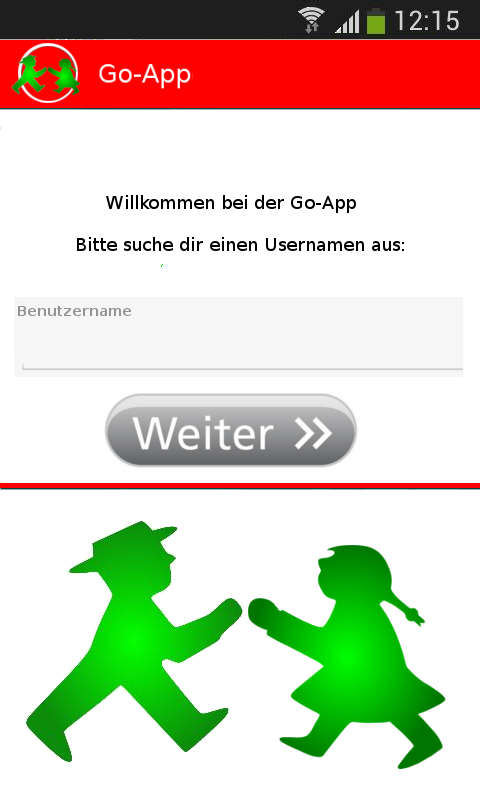
\includegraphics[scale =1]{resources/images/startansicht.png}
\end{figure}
[Bildüberschrift]Erste Startartansicht\\ \\
\textbf{Beschreibung:}\\
Erste Startansicht der App, Begrüßung des neuen Benutzers und Aufforderung an den Benutzer sich einen Benutzernamen zu wählen.\\
\textbf{Elemente:}\\
Textfeld "User name" zum Einfügen des Benutzernamens\\
"Weiter"-Button um diesen zu bestätigen\\
\textbf{Verwendung:}\\
Durch einmaliges Tippen auf das Textfeld "User name" wird die Bildschirmtastatur aktiviert und der Benutzer kann seinen gewählten Benutzernamen eingeben.\\
Durch einmaliges Tippen auf den "Weiter"-Button wird dieser Benutzername bestätigt und der Benutzer wird weiter geleitet zu der Gruppenübersicht\\ \\

\begin{figure}
	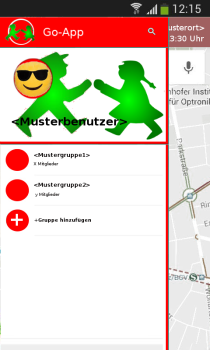
\includegraphics[scale =1]{resources/images/gruppenuebersicht.png}
\end{figure}
[Bildüberschrift]Gruppenübersicht\\ \\
\textbf{Beschreibung:}\\
Übersicht über die Gruppen, in denen der Benutzer Mitglied ist. Wenn der Benutzer das erste Mal zu dieser Ansicht gelangt, ist er in noch keiner Gruppe Mitglied und somit werden ihm auch noch keine angezeigt\\
\textbf{Elemente:}\\
Benutzernahme zur Orientierung, wie der Benutzer angemeldet ist\\
Gruppennamen zur Übersicht über die Gruppen, in denen der Benutzer Mitglied ist\\
"Gruppe hinzufügen"-Button um eine neue Gruppe hinzuzufügen
\textbf{Verwendung:}\\
(Wunschkriterium) Durch einmaliges Tippen auf den Benutzernamen wird der Benutzer weiter geleitet zu der Option Benutzername ändern\\
Durch einmaliges Tippen auf einen Gruppennamen wird der Benutzer weiter geleitet zu der Maps-Ansicht der Gruppe\\
Durch einmaliges Tippen auf den "+Gruppe hinzufügen"-Button wird der Benutzer weiter geleitet zu der Option Gruppe hinzufügen\\
Durch Streichen nach oben oder nach unten kann man durch die Gruppen scrollen, wenn es mehr sind als auf den Bildschirm passen\\
Durch Streichen von rechts nach links kann man die Gruppenansicht weg schieben und gelangt zu der zuletzt verwendeten Map\\ \\

\begin{figure}
	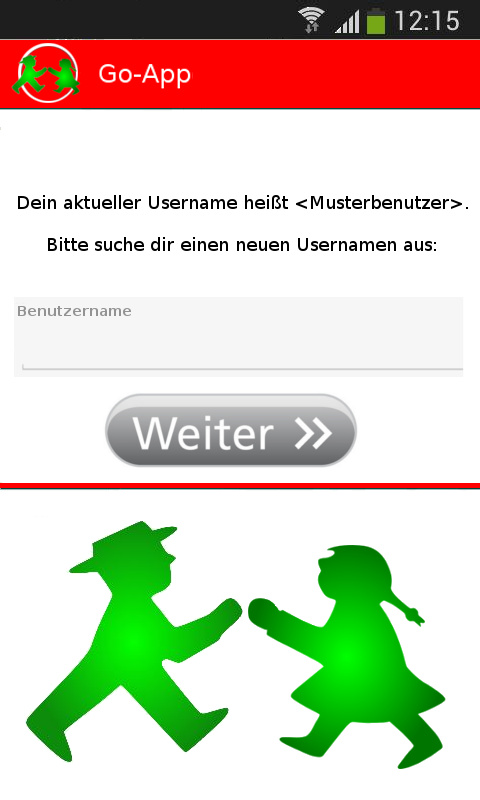
\includegraphics[scale =1]{resources/images/username_aendern.png}
\end{figure}
[Bildüberschrift]Benutzername ändern (Wunschkriterium)\\ \\
\textbf{Beschreibung:}\\
Option zum ändern des Benutzernamens, Information über den aktuellen Benutzername und Aufforderung an den Benutzer sich einen neuen Benutzernamen zu wählen\\
\textbf{Elemente:}\\
Benutzernahme zur Orientierung, wie der Benutzer angemeldet ist\\
Gruppennamen zur Übersicht über die Gruppen, in denen der Benutzer Mitglied ist\\
"Gruppe hinzufügen"-Button um eine neue Gruppe hinzuzufügen\\
\textbf{Elemente:}\\
Textfeld "User name" zum Einfügen des Benutzernamens\\
"Weiter"-Button um diesen zu bestätigen\\
\textbf{Verwendung:}\\
Durch einmaliges Tippen auf das Textfeld "User name" wird die Bildschirmtastatur aktiviert und der Benutzer kann seinen gewählten Benutzernamen eingeben.\\
Durch einmaliges Tippen auf den "Weiter"-Button wird dieser Benutzername bestätigt und der Benutzer wird weiter geleitet zu der Gruppenübersicht\\ \\

\begin{figure}
	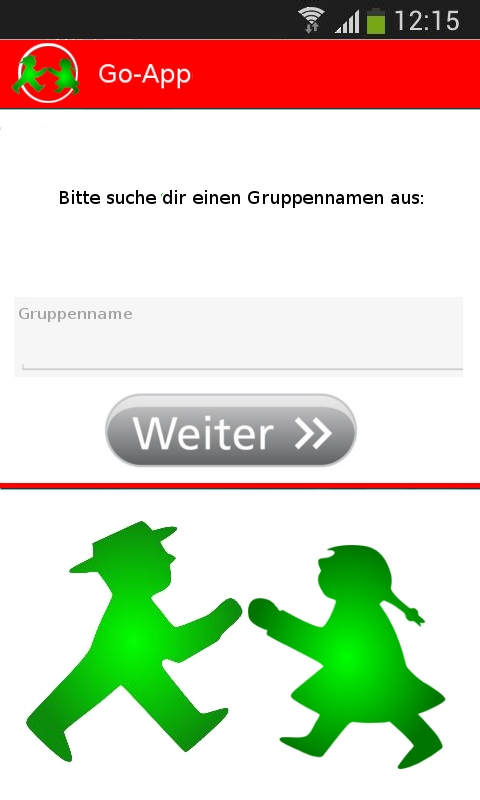
\includegraphics[scale =1]{resources/images/gruppe_erstellen.png}
\end{figure}
[Bildüberschrift]Gruppe erstellen\\ \\
\textbf{Beschreibung:}\\
Option Gruppe hinzufügen, Aufforderung an den Benutzer sich einen Gruppennamen zu wählen\\
\textbf{Elemente:}\\
Textfeld "Benutzername" zum Einfügen des Benutzernamens\\
"Weiter"-Button um diesen zu bestätigen\\
\textbf{Verwendung:}\\
Durch einmaliges Tippen auf das Textfeld "Benutzername" wird die Bildschirmtastatur aktiviert und der Benutzer kann seinen gewählten Benutzernamen eingeben.\\
Durch einmaliges Tippen auf den "Weiter"-Button wird dieser Benutzername überprüft. Ist dieser einmalig im System wird er bestätigt und der Benutzer wird weiter geleitet zu der Gruppenübersicht. Gibt es bereits eine Gruppe die den gewählten Namen trägt, öffnet sich ein kleines Fenster "Gruppenname bereits vergeben"\\ \\

\begin{figure}
	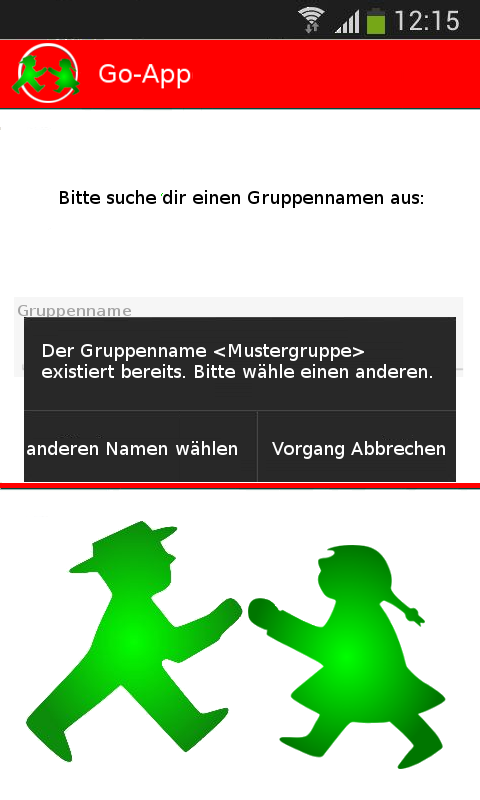
\includegraphics[scale =1]{resources/images/gruppe_erstellen_ungueltig.png}
\end{figure}
[Bildüberschrift]Gruppenname bereits vergeben\\ \\
\textbf{Beschreibung:}\\
Hinweis Gruppenname bereits vergeben. Aufforderung an den Benutzer einen anderen Gruppennamen zu wählen\\
\textbf{Elemente:}\\
"anderen Namne wählen"-Button um zurück zu der Option Gruppe erstellen zu kommen\\
"Vorgang Abbrechen"-Button um den Vorgang abzubrechen und zurück zur Gruppenübersicht zu gelangen\\
\textbf{Verwendung:}\\
Durch einmaliges Tippen auf den "anderen Namen wählen"-Button schließt sich das "Gruppenname bereits vergeben"-Fenster und der Benutzer kann erneut einen Gruppennamen auswählen.\\
Durch einmaliges Tippen auf den "Vorgang abbrechen"-Button wird der Vorgang abgebrochen und der Benutzer wird zurück geleitet zu der Gruppenübersicht.\\ \\

\begin{figure}
	
\includegraphics[scale =1]{resources/images/map_leer_Admin.png}
\end{figure}
[Bildüberschrift]Map-Ansicht der Gruppe (leer) für den Gruppenadministrator\\ \\
\textbf{Beschreibung:}\\
Map-Ansicht der Gruppe. Wenn der Gruppenadministrator das erste Mal zu dieser Ansicht gelangt, hat er noch keine Treffen erstellt und somit wird ihm auch noch eine leere Map angezeigt. Ebenso wenn er noch kein aktuelles Treffen erstellt hat.\\
\textbf{Elemente:}\\
"Gruppenname"-Button um zu den Gruppendetails zu gelangen\\
"neues Treffen erstellen"-Button um ein neues Treffen zu erstellen\\
"Hier suchen"-Textfeld um einen Ort auf der Karte zu suchen\\
Lupen-Button um die Suche zu starten\\
Handle links unten in der Ecke um die Gruppenansicht wieder herauszuziehen\\
\textbf{Verwendung:}\\
Durch einmaliges Tippen auf den "Gruppenname"-Button wird der Gruppenadministrator weiter geleitet zu der Ansicht "Gruppendeteils Gruppenadministrator".\\
Durch einmaliges Tippen auf den "neues Treffen erstellen"-Button wird der Gruppenadministrator weiter geleitet zu der Option "Treffpunkt erstellen"\\
Durch einmaliges Tippen auf das Textfeld "Hier suchen" wird die Bildschirmtastatur aktiviert und der Gruppenadministrator kann seinen gewählten Ort eingeben.\\
Durch einmaliges Tippen auf den Lupen-Button wird eine Suche nach dem gewählten Ort gestartet und die Ergebnisse dem Gruppenadministrator angezeigt\\
Durch Streichen von links nach rechts über den Hanlde-Button kann der Gruppenadministrator die Gruppenansicht wieder herausziehen\\ \\

\begin{figure}
	
\includegraphics[scale =1]{resources/images/map_leer.png}
\end{figure}
[Bildüberschrift]Map-Ansicht der Gruppe (leer) für alle Gruppenmitglieder\\ \\
\textbf{Beschreibung:}\\
Map-Ansicht der Gruppe. Wenn der Gruppenadministrator noch kein aktuelles Treffen erstellt hat, wird jedem Gruppenmitglied noch eine leere Map angezeigt.\\
\textbf{Elemente:}\\
"Gruppenname"-Button um zu den Gruppendetails zu gelangen\\
"kein aktuelles Treffen"-Button nicht aktiviert\\
"Hier suchen"-Textfeld um einen Ort auf der Karte zu suchen\\
Lupen-Button um die Suche zu starten\\
Handle links unten in der Ecke um die Gruppenansicht wieder herauszuziehen\\
\textbf{Verwendung:}\\
Durch einmaliges Tippen auf den "Gruppenname"-Button wird das Gruppenmitglied weiter geleitet zu der Ansicht "Gruppenmitglieder".\\
Der "kein aktuelles Treffen"-Button ist in dieser Ansicht für Gruppenmitglieder nicht aktiviert\\
Durch einmaliges Tippen auf das Textfeld "Hier suchen" wird die Bildschirmtastatur aktiviert und das Gruppenmitglied kann seinen gewählten Ort eingeben.\\
Durch einmaliges Tippen auf den Lupen-Button wird eine Suche nach dem gewählten Ort gestartet und die Ergebnisse dem Gruppenmitglied angezeigt\\
Durch Streichen von links nach rechts über den Hanlde-Button kann das Gruppenmitglied die Gruppenansicht wieder herausziehen\\ \\

\begin{figure}
	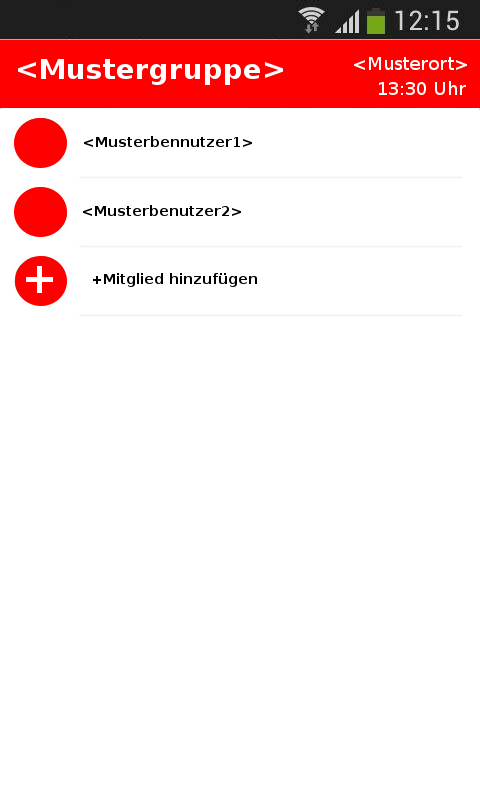
\includegraphics[scale =1]{resources/images/gruppendetails_Admin.png}
\end{figure}
[Bildüberschrift]Übersicht über die Gruppenmitglieder für den Gruppenadministrator\\ \\
\textbf{Beschreibung:}\\
Übersicht über die Mitglieder dieser Gruppe. Wenn der Gruppenadministrator das erste Mal zu dieser Ansicht gelangt, ist außer ihm noch kein weiteres Mitglied in dieser Gruppe und somit werden ihm auch noch keine weiteren angezeigt\\
\textbf{Elemente:}\\
"Gruppenname"-Button zur Übersicht, welcher Gruppe der Gruppenadministrator bearbeitet und um zurück zur Map-Ansicht der Gruppe zu gelangen\\
"neues Treffen erstellen"-Button bzw. Uhrzeit-Button um ein neues Treffen zu erstellen\\
Mitgliedernamen zur Übersicht über die Mitglied der Gruppe\\
"Mitglied hinzufügen"-Button um ein neues Mitglied einzuladen
\textbf{Verwendung:}\\
Durch einmaliges Tippen auf den "Gruppenname"-Button wird der Gruppenadministrator zurück geleitet zu der Map-Ansicht der Gruppe\\
"neues Treffen erstellen"-Button bzw. Uhrzeit-Button hat die selbe Funktion wie in der Map-Ansicht der Gruppe\\
Durch einmaliges Tippen auf den "+Mitglied hinzufügen"-Button öffnet sich das Fenster "Link versenden"\\ \\

\begin{figure}
	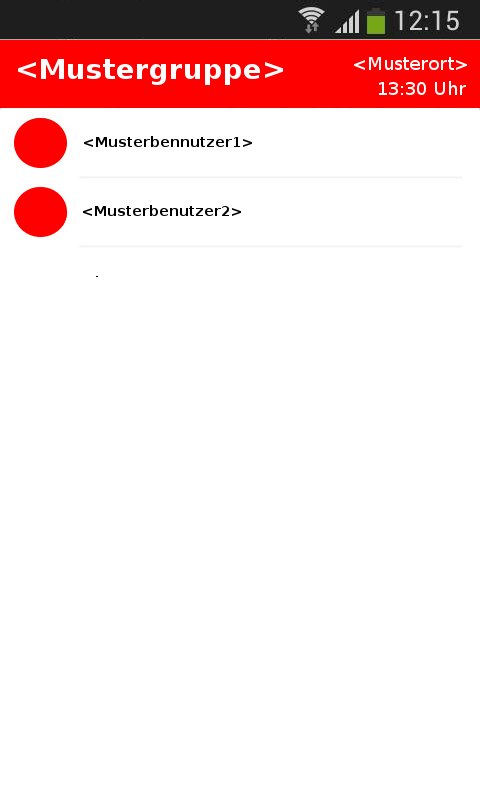
\includegraphics[scale =1]{resources/images/gruppendetails.png}
\end{figure}
[Bildüberschrift]Übersicht über die Gruppenmitglieder für alle Gruppenmiglieder\\ \\
\textbf{Beschreibung:}\\
Übersicht über die Mitglieder dieser Gruppe.\\
\textbf{Elemente:}\\
"Gruppenname"-Button zur Übersicht, welcher Gruppe das Gruppenmitglied  bearbeitet und um zurück zur Map-Ansicht der Gruppe zu gelangen\\
"kein aktuelles Treffen"-Button bzw. Uhrzeit-Button um ein neues Treffen zu erstellen\\
Mitgliedernamen zur Übersicht über die Mitglied der Gruppe\\
\textbf{Verwendung:}\\
Durch einmaliges Tippen auf den "Gruppenname"-Button wird der Gruppenadministrator zurück geleitet zu der Map-Ansicht der Gruppe\\
"kein aktuelles Treffen"-Button bzw. Uhrzeit-Button hat die selbe Funktion wie in der Map-Ansicht der Gruppe\\

\begin{figure}
	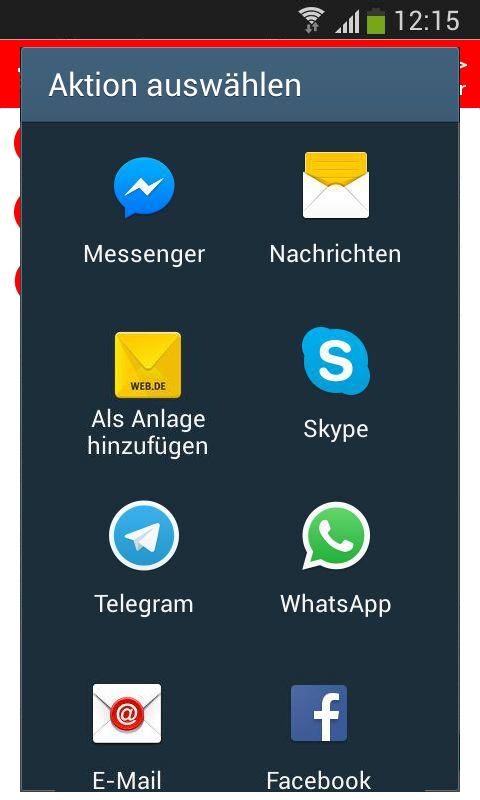
\includegraphics[scale =1]{resources/images/link_versenden.png}
\end{figure}
[Bildüberschrift]Link versenden\\ \\
\textbf{Beschreibung:}\\
Übersicht über verschiedene Kommunikationswege, die verwendet werden können um andere Mitglieder in die Gruppe einzuladen.\\
\textbf{Elemente:}\\
beliebig viele Button der Kommunikationswegen, die der Gruppenadministrator auf seinem Android-Gerät installiert hat\\
\textbf{Verwendung:}\\
Durch einmaliges Tippen auf einen der Button wird der Gruppenadministrator weiter geleitet zu der ausgewählten Applikation über die er dann den neu generierten Gruppen-Einladungs-Link versenden kann\\ \\

\begin{figure}
	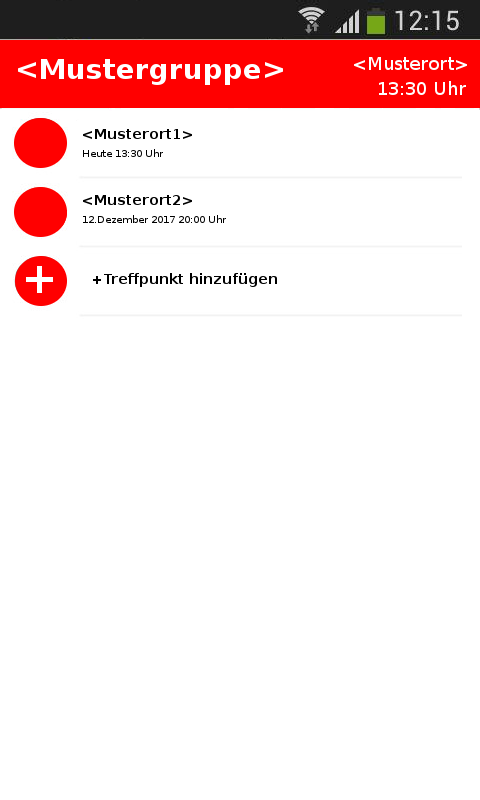
\includegraphics[scale =1]{resources/images/treffpunktuebersicht_Admin.png}
\end{figure}
[Bildüberschrift]Übersicht über die bevorstehenden Treffpunkte für den Gruppenadministrator\\ \\
\textbf{Beschreibung:}\\
Übersicht über die bevorstehenden Treffpunkte dieser Gruppe. Wenn der Gruppenadministrator das erste Mal zu dieser Ansicht gelangt, hat er noch keine Treffen erstellt und somit wird ihm auch noch keines angezeigt. Ebenso wenn er noch kein aktuelles Treffen erstellt hat.\\
\textbf{Elemente:}\\
"Gruppenname"-Button zur Übersicht, welcher Gruppe der Gruppenadministrator bearbeitet und um zu den Gruppendetails zu kommen\\
"neues Treffen erstellen"-Button bzw. Uhrzeit-Button um zurück zur Map-Ansicht der Gruppe zu gelangen\\
Treffen mit Zielort, Uhrzeit und (Wunschkriterium) Tag zur Übersicht über die bereits erstellten Treffen der Gruppe\\
"Treffen hinzufügen"-Button um ein neues Treffen zu erstellen
\textbf{Verwendung:}\\
Der "Gruppenname"-Button  hat die selbe Funktion wie in der Map-Ansicht der Gruppe\\
Durch einmaliges Tippen auf den "neues Treffen erstellen"-Button bzw. Uhrzeit-Button wird der Gruppenadministrator zurück geleitet zu der Map-Ansicht der Gruppe\\
Durch langes Halten auf ein Treffen, kommt der Gruppenadministrator zu den Optionen "Treffen bearbeiten" und "Treffen löschen"
Durch einmaliges Tippen auf den "+Treffen hinzufügen"-Button wird der Gruppenadministrator weiter geleitet zu der Option "Treffen erstellen"\\ \\

\begin{figure}
	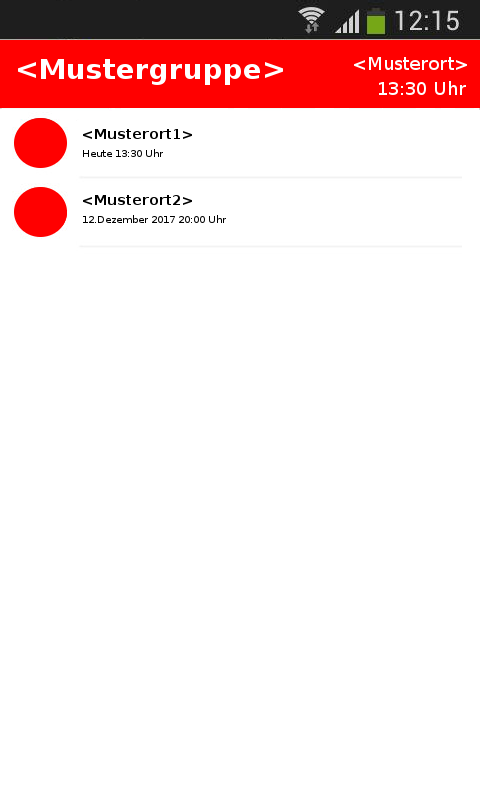
\includegraphics[scale =1]{resources/images/treffpunktuebersicht.png}
\end{figure}
[Bildüberschrift]Übersicht über die bevorstehenden Treffpunkte für alle Gruppenmitglieder\\ \\
\textbf{Beschreibung:}\\
Übersicht über die bevorstehenden Treffpunkte dieser Gruppe. Wenn der Gruppenadministrator noch kein aktuelles Treffen erstellt hat, wird jedem Gruppenmitglied auch noch keines angezeigt.\\
\textbf{Elemente:}\\
"Gruppenname"-Button zur Übersicht, welche Gruppe sich hier verabredet und um zu den Gruppendetails zu kommen\\
"kein aktuelles Treffen"-Button bzw. Uhrzeit-Button um zurück zur Map-Ansicht der Gruppe zu gelangen\\
Treffen mit Zielort, Uhrzeit und (Wunschkriterium) Tag zur Übersicht über die bereits festgelegten Treffen der Gruppe\\
\textbf{Verwendung:}\\
Der "Gruppenname"-Button  hat die selbe Funktion wie in der Map-Ansicht der Gruppe\\
Durch einmaliges Tippen auf den "kein aktuelles Treffen"-Button bzw. Uhrzeit-Button wird das Gruppenmitglied zurück geleitet zu der Map-Ansicht der Gruppe\\ \\

\begin{figure} 
	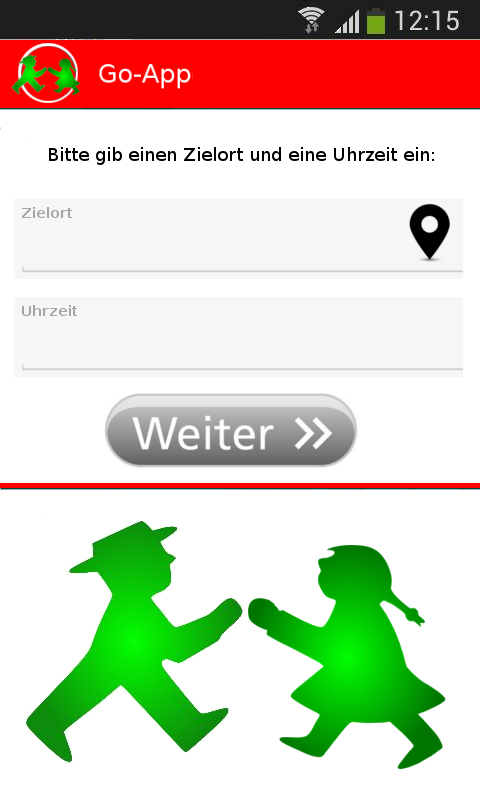
\includegraphics[scale =1]{resources/images/treffpunkt_erstellen.png}
\end{figure}
[Bildüberschrift]Treffen erstellen \\ \\
\textbf{Beschreibung:}\\
Option zum Erstellen eines neuen Treffens, Aufforderung an den Gruppenadministrator einen Zielort und eine Uhrzeit zu wählen.\\
\textbf{Elemente:}\\
Textfeld "Zielort" zum Einfügen des Zielortes\\
Map-Symbol-Button zum Auswählen des Zielortes per Map\\
Textfeld "Uhrzeit" zum Einfügen der Uhrzeit\\
"Weiter"-Button um diese zu bestätigen\\
\textbf{Verwendung:}\\
Durch einmaliges Tippen auf das Textfeld "Zielort" wird die Bildschirmtastatur aktiviert und der Gruppenadministrator kann seinen gewählten Zielort eingeben.\\
Alternativ: durch einmaliges Tippen auf den Map-Symbol-Button wird der Gruppenadministrator weiter geleitet zu der Map-Ansicht und kann dort durch einmaliges Tippen auf einen Ort diesen als Zielort eingeben\\
Durch einmaliges Tippen auf das Textfeld "Uhrzeit" wird die Bildschirm-Zahlentastatur aktiviert und der Gruppenadministrator kann seine gewählte Zielzeit eingeben.\\
Durch einmaliges Tippen auf den "Weiter"-Button werden dieser Zielort und diese Uhrzeit überprüft. Gibt es den Zielort und diese Uhrzeit, werden diese bestätigt und der Gruppenadministrator wird weiter geleitet zu der Übersicht über die bevorstehenden Treffen. Gibt es diesen Ort nicht, öffnet sich ein kleines Fenster "Zielort ungültig". Gibt es diese Zeit nicht, öffnet sich ein kleines Fenster "Uhrzeit ungültig".\\ \\

\begin{figure}
	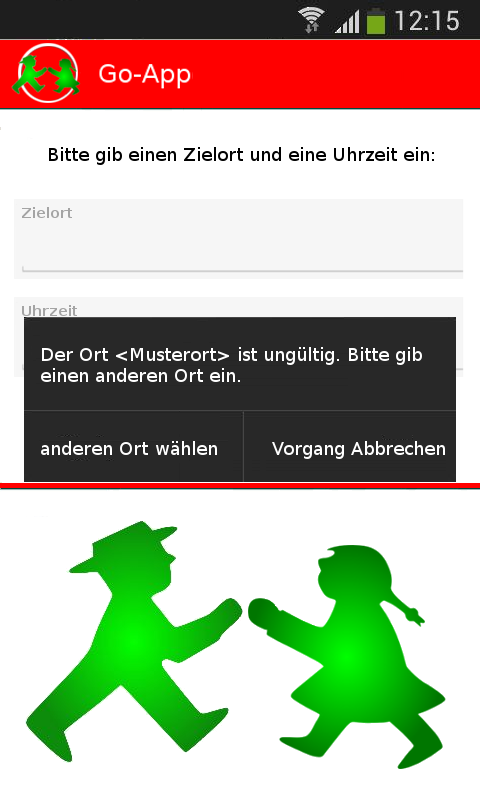
\includegraphics[scale =1]{resources/images/treffpunkt_erstellen_ungueltig_Ort.png}
\end{figure}
[Bildüberschrift]Zielort ungültig\\ \\
\textbf{Beschreibung:}\\
Hinweis Zielort ist ungültig. Aufforderung an den Gruppenadministrator einen anderen Zielort zu wählen\\
\textbf{Elemente:}\\
"anderen Ort wählen"-Button um zurück zu der Option Treffen erstellen zu kommen\\
"Vorgang Abbrechen"-Button um den Vorgang abzubrechen und zurück Übersicht über die bevorstehenden Treffen zu gelangen\\
\textbf{Verwendung:}\\
Durch einmaliges Tippen auf den "anderen Ort wählen"-Button schließt sich das "Gruppenname bereits vergeben"-Fenster und der Benutzer kann erneut einen Zielort auswählen.\\
Durch einmaliges Tippen auf den "Vorgang abbrechen"-Button wird der Vorgang abgebrochen und der Benutzer wird zurück geleitet zu der Übersicht über die bevorstehenden Treffen.\\ \\

\begin{figure}
	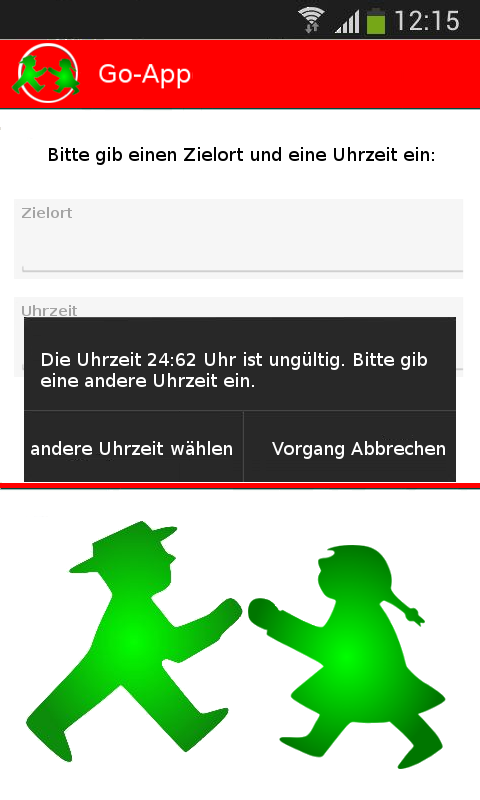
\includegraphics[scale =1]{resources/images/treffpunkt_erstellen_ungueltig_Zeit.png}
\end{figure}
[Bildüberschrift]Uhrzeit ungültig\\ \\
\textbf{Beschreibung:}\\
Hinweis Uhrzeit ist ungültig. Aufforderung an den Gruppenadministrator eine andere Uhrzeit zu wählen\\
\textbf{Elemente:}\\
"anderen Uhrzeit wählen"-Button um zurück zu der Option Treffen erstellen zu kommen\\
"Vorgang Abbrechen"-Button um den Vorgang abzubrechen und zurück Übersicht über die bevorstehenden Treffen zu gelangen\\
\textbf{Verwendung:}\\
Durch einmaliges Tippen auf den "anderen Uhrzeit wählen"-Button schließt sich das "Gruppenname bereits vergeben"-Fenster und der Benutzer kann erneut eine Uhrzeit auswählen.\\
Durch einmaliges Tippen auf den "Vorgang abbrechen"-Button wird der Vorgang abgebrochen und der Benutzer wird zurück geleitet zu der Übersicht über die bevorstehenden Treffen.\\ \\

\begin{figure}
	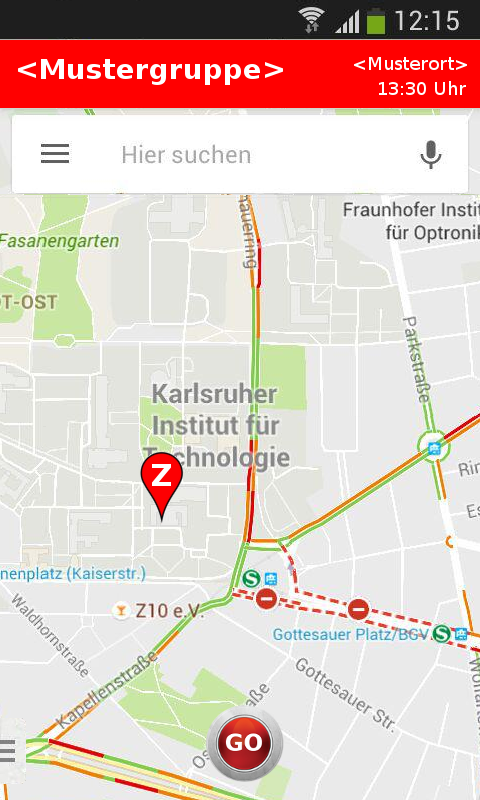
\includegraphics[scale =1]{resources/images/map.png}
\end{figure}
[Bildüberschrift]Map-Ansicht der Gruppe - Treffpunkt festgelegt\\ \\
\textbf{Beschreibung:}\\
Map-Ansicht der Gruppe mit festgelegtem Treffpunkt. Allen Gruppenmitgliedern wird in dieser Ansicht nicht nur die Map angezeigt, sondern auch der Zielort und die Uhrzeit des nächsten festgelegten Treffpunktes, außerdem noch auf der Map der Zielort mit einer Stecknadel beschriftet mit "Z".\\
\textbf{Elemente:}\\
"Gruppenname"-Button um zu den Gruppendetails zu gelangen\\
"Zielort - Uhrzeit"-Button zur Orientierung wann und wo das nächste Treffen festgelegt ist und um zu der Option "Übersicht über die bevorstehenden Treffpunkte" zu gelangen.\\
"Hier suchen"-Textfeld um einen Ort auf der Karte zu suchen\\
Lupen-Button um die Suche zu starten\\
Handle links unten in der Ecke um die Gruppenansicht wieder herauszuziehen\\
Aktiver "Go"-Button um anzuzeigen, wann man los geht
\textbf{Verwendung:}\\
Durch einmaliges Tippen auf den "Gruppenname"-Button wird das Gruppenmitglied weiter geleitet zu der Ansicht "Gruppendeteils".\\
Durch einmaliges Tippen auf den "Zielort - Uhrzeit"-Button wird das Gruppenmitglied weiter geleitet zu der Option "Übersicht über die bevorstehenden Treffpunkte"\\
Durch einmaliges Tippen auf das Textfeld "Hier suchen" wird die Bildschirmtastatur aktiviert und das Gruppenmitglied kann seinen gewählten Ort eingeben.\\
Durch einmaliges Tippen auf den Lupen-Button wird eine Suche nach dem gewählten Ort gestartet und die Ergebnisse dem Gruppenmitglied angezeigt\\
Durch Streichen von links nach rechts über den Hanlde-Button kann das Gruppenmitglied die Gruppenansicht wieder herausziehen\\
Durch einmaliges Tippen auf den "Go"-Button sendet das Gruppenmitglied seinen Standort in regelmäßigen Zeitabständen zu den anderen Gruppenmitgliedern und erhält auch alle nötigen Informationen über diese (Ansicht: "Map-Ansicht der Gruppe - treffen")\\ \\

\begin{figure}
	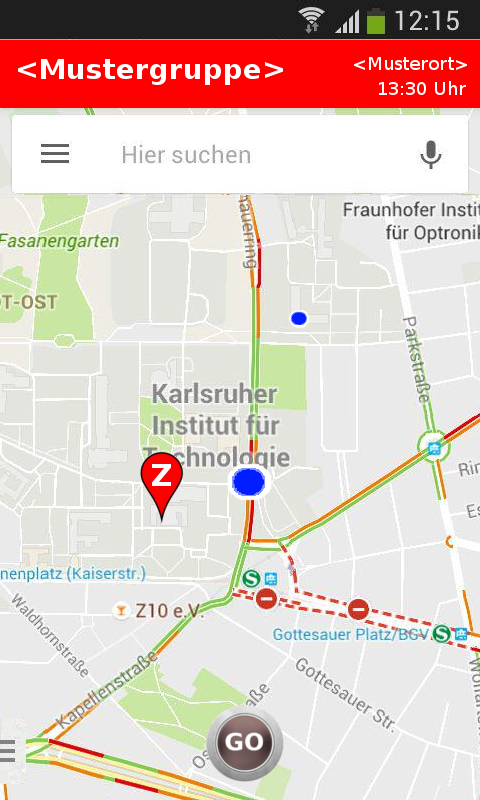
\includegraphics[scale =1]{resources/images/map_Go.png}
\end{figure}
[Bildüberschrift]Map-Ansicht der Gruppe - treffen\\ \\
\textbf{Beschreibung:}\\
Map-Ansicht der Gruppe wenn der "Go"-Button schon gedrückt ist. Allen Gruppenmitgliedern wird in dieser Ansicht nicht nur die Map angezeigt, sondern auch der Zielort und die Uhrzeit des nächsten festgelegten Treffpunktes, außerdem noch auf der Map der Zielort mit einer Stecknadel beschriftet mit "Z" und die Standorte der anderen Gruppenmitglieder durch blaue Kreise. Je größer ein Kreis, desto mehr Mitglieder befinden sich an dem gleichen Standort.\\
\textbf{Elemente:}\\
"Gruppenname"-Button um zu den Gruppendetails zu gelangen\\
"Zielort - Uhrzeit"-Button zur Orientierung wann und wo das nächste Treffen festgelegt ist und um zu der Option "Übersicht über die bevorstehenden Treffpunkte" zu gelangen.\\
"Hier suchen"-Textfeld um einen Ort auf der Karte zu suchen\\
Lupen-Button um die Suche zu starten\\
Handle links unten in der Ecke um die Gruppenansicht wieder herauszuziehen\\
Deaktiver "Go"-Button um das Versenden seines Standortes zu stoppen\\
\textbf{Verwendung:}\\
Durch einmaliges Tippen auf den "Gruppenname"-Button wird das Gruppenmitglied weiter geleitet zu der Ansicht "Gruppendeteils".\\
Durch einmaliges Tippen auf den "Zielort - Uhrzeit"-Button wird das Gruppenmitglied weiter geleitet zu der Option "Übersicht über die bevorstehenden Treffpunkte"\\
Durch einmaliges Tippen auf das Textfeld "Hier suchen" wird die Bildschirmtastatur aktiviert und das Gruppenmitglied kann seinen gewählten Ort eingeben.\\
Durch einmaliges Tippen auf den Lupen-Button wird eine Suche nach dem gewählten Ort gestartet und die Ergebnisse dem Gruppenmitglied angezeigt\\
Durch Streichen von links nach rechts über den Hanlde-Button kann das Gruppenmitglied die Gruppenansicht wieder herausziehen\\
Durch einmaliges Tippen auf den "Go"-Button wird dieser wieder aktiv und das Senden des Standortes des Gruppenmitgliedes wird gestoppt. Außerdem kann das Gruppenmitglied dann nicht mehr die Standorte der anderen Gruppenmitglieder sehen (Ansicht: "Map-Ansicht der Gruppe - Treffen festgelegt")\\ \\